\documentclass[]{article}

\usepackage{
	amsmath, 
	amssymb,
	float,
	graphicx,
	bera,
	parskip,
	booktabs,
	multirow,
	xcolor,
	colortbl
}

\graphicspath{ {Images/} }

\title{Assignment 4}
\author{
	Daniel Bok \\
	ESD \\
	1001049 \\
	daniel\_bok@mymail.sutd.edu.sg 
	\and
	Wong Yan Yee\\ 
	ISTD \\
	1001212 \\
	yanyee\_wong@mymail.sutd.edu.sg
	\and
	Clement Tan \\
	ESD \\
	1000948 \\
	clement\_tan@mymail.sutd.edu.sg
}
\date{\today}

\begin{document}
	
\maketitle

\newpage
\section*{Question 7.3}

\subsection*{A: Forming The Adjacency Matrix}

\begin{figure}[H]
	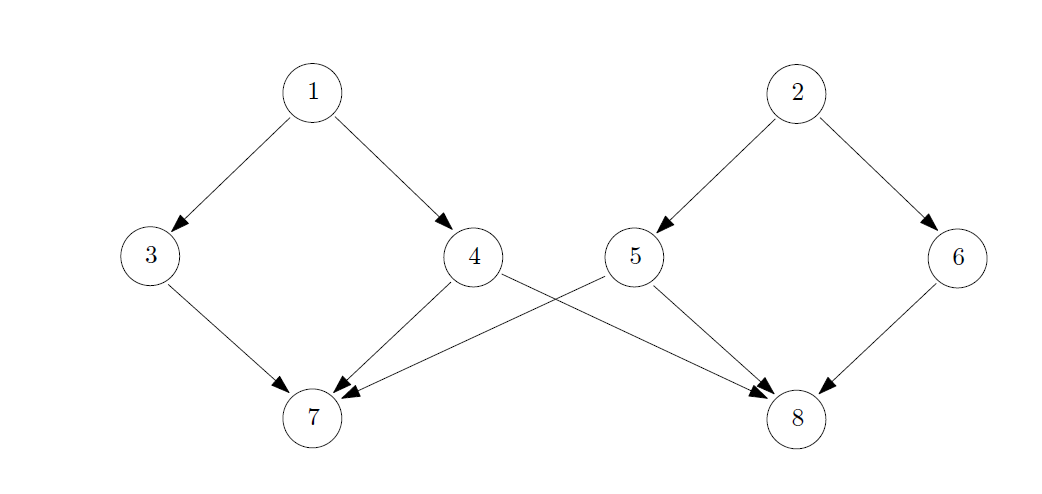
\includegraphics[width=\linewidth]{7-16.png}
	\caption{Network Graph} 
	\label{Q7.3 Network Graph 1}
\end{figure}

Given the network graph in Figure \ref{Q7.3 Network Graph 1}, the adjacency matrix $\mathbf{A}$ is given by
\begin{gather*}
	\mathbf{A} = \begin{bmatrix}
		0 & 0 & 1 & 1 & 0 & 0 & 0 & 0 \\
		0 & 0 & 0 & 0 & 1 & 1 & 0 & 0 \\
		0 & 0 & 0 & 0 & 0 & 0 & 1 & 0 \\
		0 & 0 & 0 & 0 & 0 & 0 & 1 & 1 \\
		0 & 0 & 0 & 0 & 0 & 0 & 1 & 1 \\
		0 & 0 & 0 & 0 & 0 & 0 & 0 & 1 \\
		0 & 0 & 0 & 0 & 0 & 0 & 0 & 0 \\
		0 & 0 & 0 & 0 & 0 & 0 & 0 & 0
	\end{bmatrix}
\end{gather*}

\subsection*{B: What is Matrix C?}

\begin{align*}
	\mathbf{C} &= \mathbf{A}^T\mathbf{A} \\
		&= \begin{bmatrix}
			0 & 0 & 0 & 0 & 0 & 0 & 0 & 0 \\
			0 & 0 & 0 & 0 & 0 & 0 & 0 & 0 \\
			0 & 0 & 1 & 1 & 0 & 0 & 0 & 0 \\
			0 & 0 & 1 & 1 & 0 & 0 & 0 & 0 \\
			0 & 0 & 0 & 0 & 1 & 1 & 0 & 0 \\
			0 & 0 & 0 & 0 & 1 & 1 & 0 & 0 \\
			0 & 0 & 0 & 0 & 0 & 0 & 3 & 2 \\
			0 & 0 & 0 & 0 & 0 & 0 & 2 & 3
		\end{bmatrix}
\end{align*}

The physical interpretation of $C_{ij}$ is the number of papers which cited paper $i$ and paper $j$ together. We notice that $C_{78} = C_{87} = 2$ because papers 4 and 5 cited both of them together. The same goes for $C_{56}$ and others.

We thus notice that $C_{78} > C_{75}$ because no papers which cited paper 5 cited paper 7 and vice versa. Thus $C_{75} = 0$.

\subsection*{C: Raising Matrix A}

\begin{align*}
	\mathbf{A}^2 &= \begin{bmatrix}
		0 & 0 & 0 & 0 & 0 & 0 & 2 & 1 \\
		0 & 0 & 0 & 0 & 0 & 0 & 1 & 2 \\
		0 & 0 & 0 & 0 & 0 & 0 & 0 & 0 \\
		0 & 0 & 0 & 0 & 0 & 0 & 0 & 0 \\
		0 & 0 & 0 & 0 & 0 & 0 & 0 & 0 \\
		0 & 0 & 0 & 0 & 0 & 0 & 0 & 0 \\
		0 & 0 & 0 & 0 & 0 & 0 & 0 & 0 \\
		0 & 0 & 0 & 0 & 0 & 0 & 0 & 0
	\end{bmatrix} \\
	\mathbf{A}^3 &= \begin{bmatrix}
		0 & 0 & 0 & 0 & 0 & 0 & 0 & 0 \\
		0 & 0 & 0 & 0 & 0 & 0 & 0 & 0 \\
		0 & 0 & 0 & 0 & 0 & 0 & 0 & 0 \\
		0 & 0 & 0 & 0 & 0 & 0 & 0 & 0 \\
		0 & 0 & 0 & 0 & 0 & 0 & 0 & 0 \\
		0 & 0 & 0 & 0 & 0 & 0 & 0 & 0 \\
		0 & 0 & 0 & 0 & 0 & 0 & 0 & 0 \\
		0 & 0 & 0 & 0 & 0 & 0 & 0 & 0
	\end{bmatrix}
\end{align*}

In general, the entries $a_ij$ in the matrix $\mathbf{A}^M$ refers to the number of ways to get from node $i$ to node $j$ in $M$ steps. $\mathbf{A}^3$ is a zero-matrix because there are no connections of length 3. 

\newpage

\section*{Question 8.1}

\subsection*{Degree, Closeness, and Eigenvector centrality}

\begin{table}[htbp]
	\centering
	\caption{Centrality}
	\begin{tabular}{|cccc|}
		\toprule
		\rowcolor[rgb]{ .267,  .447,  .769} \multicolumn{1}{|l}{\textcolor[rgb]{ 1,  1,  1}{\textbf{Nodes}}} & \multicolumn{1}{l}{\textcolor[rgb]{ 1,  1,  1}{\textbf{Degree}}} & \multicolumn{1}{l}{\textcolor[rgb]{ 1,  1,  1}{\textbf{Closeness}}} & \multicolumn{1}{l|}{\textcolor[rgb]{ 1,  1,  1}{\textbf{Eigenvector}}} \\
		\midrule
		1     & 3     & 0.800 & 0.4558 \\
		\midrule
		2     & 2     & 0.667 & 0.3192 \\
		\midrule
		3     & 3     & 0.800 & 0.4912 \\
		\midrule
		4     & 3     & 0.800 & 0.4912 \\
		\midrule
		5     & 3     & 0.800 & 0.4558 \\
		\bottomrule
	\end{tabular}
	\label{table:DCE_Centrality}
\end{table}

\subsection*{Node Betweenness Centrality}

\begin{table}[htbp]
	\centering
	\caption{Betweenness Centrality of Node 2 and 3}
	\begin{tabular}{|cc|}
		\toprule
		\rowcolor[rgb]{ .267,  .447,  .769} \multicolumn{1}{|l}{\textcolor[rgb]{ 1,  1,  1}{\textbf{Node}}} & \multicolumn{1}{l|}{\textcolor[rgb]{ 1,  1,  1}{\textbf{Betweenness}}} \\
		\midrule
		2     & 0.0625 \\
		\midrule
		3     & 0.0556 \\
		\bottomrule
	\end{tabular}
	\label{table:Betweenness_Centrality}
\end{table}

\subsection*{Link Betweenness Centrality}

\begin{table}[htbp]
	\centering
	\caption{Link Betweenness Centrality}
	\begin{tabular}{|cc|}
		\toprule
		\rowcolor[rgb]{ .267,  .447,  .769} \multicolumn{1}{|l}{\textcolor[rgb]{ 1,  1,  1}{\textbf{Links}}} & \multicolumn{1}{l|}{\textcolor[rgb]{ 1,  1,  1}{\textbf{Betweenness}}} \\
		\midrule
		(2, 5) & 2.33 \\
		\midrule
		(3, 4) & 1 \\
		\bottomrule
	\end{tabular}
	\label{table:Link_Betweenness_Centrality}
\end{table}


\newpage
\section*{Question 8.2}

\subsection*{Only Node 1 is infected}
When only Node 1 is infected (at state 1) initially, the contagion effect in the long run is given by

\begin{table}[htbp]
	\centering
	\caption{Long Run Contagion Effect 1}
	\begin{tabular}{|ccccccccc|}
		\toprule
		\rowcolor[rgb]{ .267,  .447,  .769} \textcolor[rgb]{ 1,  1,  1}{\textbf{Node}} & \textcolor[rgb]{ 1,  1,  1}{\textbf{1}} & \textcolor[rgb]{ 1,  1,  1}{\textbf{2}} & \textcolor[rgb]{ 1,  1,  1}{\textbf{3}} & \textcolor[rgb]{ 1,  1,  1}{\textbf{4}} & \textcolor[rgb]{ 1,  1,  1}{\textbf{5}} & \textcolor[rgb]{ 1,  1,  1}{\textbf{6}} & \textcolor[rgb]{ 1,  1,  1}{\textbf{7}} & \textcolor[rgb]{ 1,  1,  1}{\textbf{8}} \\
		\midrule
		\textbf{Infected?} & 1     & 1     & 0     & 0     & 0     & 0     & 1     & 1 \\
		\bottomrule
	\end{tabular}
	\label{table:contagion_1}
\end{table}

1 in the \textbf{"Infected?"} row represents that the node will be infected in the long run.

\subsection*{Only Node 3 is infected}
When only Node 1 is infected (at state 1) initially, the contagion effect in the long run is given by

\begin{table}[htbp]
	\centering
	\caption{Long Run Contagion Effect 2}
	\begin{tabular}{|ccccccccc|}
		\toprule
		\rowcolor[rgb]{ .267,  .447,  .769} \textcolor[rgb]{ 1,  1,  1}{\textbf{Node}} & \textcolor[rgb]{ 1,  1,  1}{\textbf{1}} & \textcolor[rgb]{ 1,  1,  1}{\textbf{2}} & \textcolor[rgb]{ 1,  1,  1}{\textbf{3}} & \textcolor[rgb]{ 1,  1,  1}{\textbf{4}} & \textcolor[rgb]{ 1,  1,  1}{\textbf{5}} & \textcolor[rgb]{ 1,  1,  1}{\textbf{6}} & \textcolor[rgb]{ 1,  1,  1}{\textbf{7}} & \textcolor[rgb]{ 1,  1,  1}{\textbf{8}} \\
		\midrule
		\textbf{Infected?} & 1     & 1     & 1     & 1     & 1     & 1     & 1     & 1 \\
		\bottomrule
	\end{tabular}
	\label{table:contagion_2}
\end{table}

\subsection*{Reasons for differences}

The inner cluster (Nodes 3, 4, 5, 6) has a cluster density of 75\%. This means that external nodes only has a 25\% level of influence on this cluster. The threshold value of 0.3 (or 30\%) is too high and thus it is impossible to penetrate this cluster as seen in Part A.

In Part B, when Node 3 (which belongs in the cluster) is infected, it allowed the nodes within the cluster to be influenced. Thus every node in the network was eventually infected.

\newpage
\section*{Question 8.3}

\begin{figure}[H]
	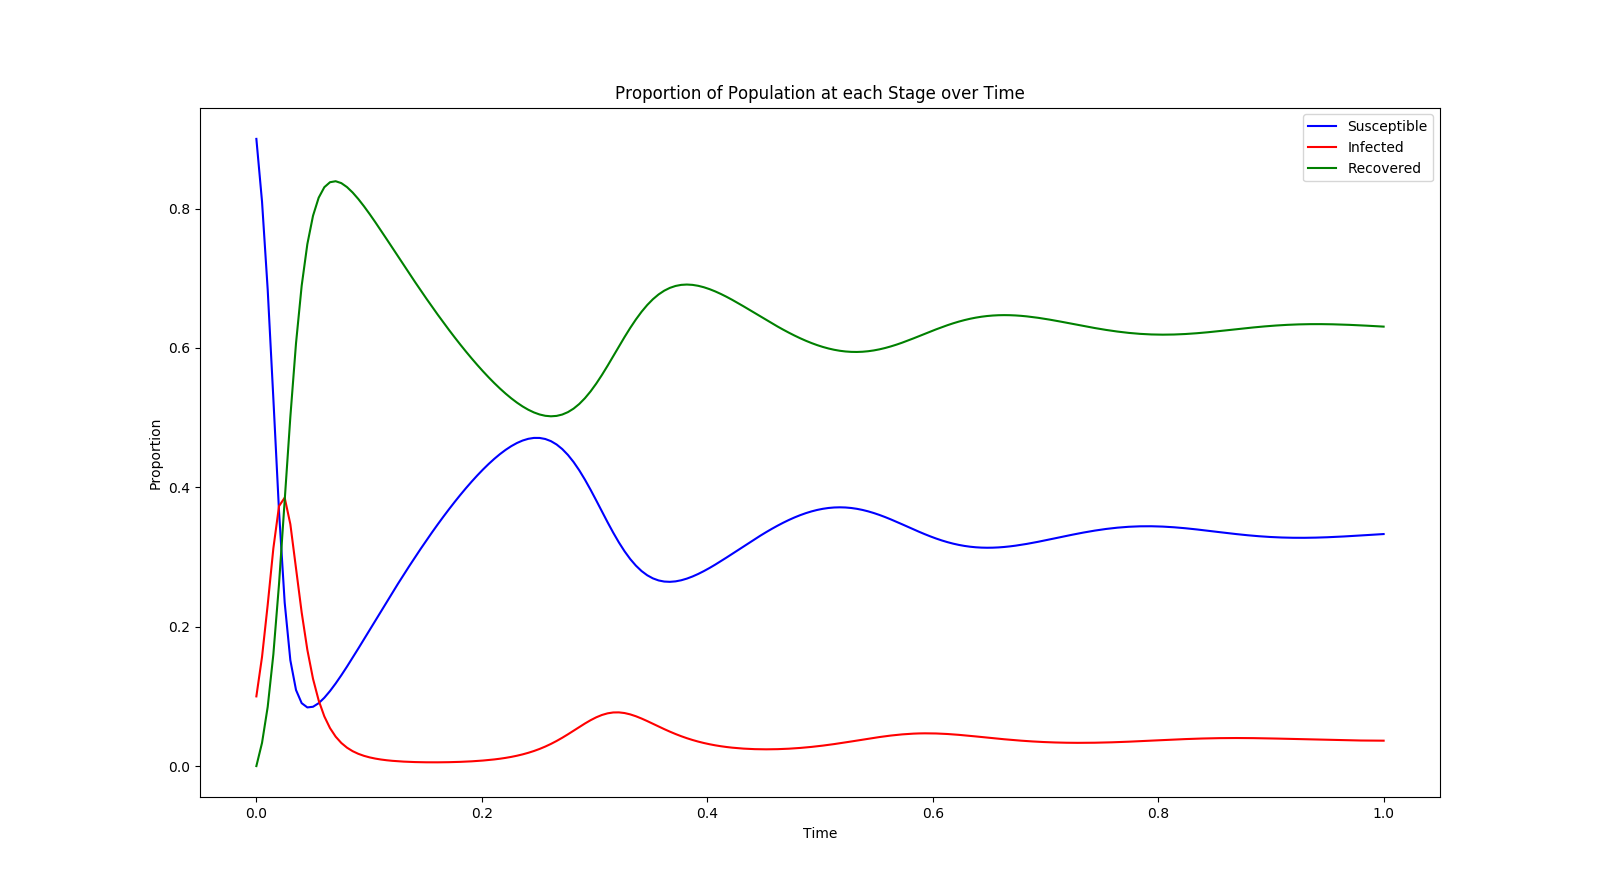
\includegraphics[width=\linewidth]{8-3.png}
	\caption{SIR Evolution Graph} 
	\label{Q8.3 SIR Graph}
\end{figure}

As can be seen from Figure \ref{Q8.3 SIR Graph}, we notice that there is initially a lot of fluctuation. However, by around 0.8 (percentage over entire timespan) of the evolution, the 3 stages converge to a stable value.

The first thing we notice is that
\[
	\frac{dS(t)}{dt} + \frac{dI(t)}{dt} + \frac{dR(t)}{dt} = 0
\]
Thus there is no change in the overall population at any time. Since such is the case and given the values of the parameters $\beta$, $\nu$ and $\gamma$, the solution is bound to converge as evidenced in Figure \ref{Q8.3 SIR Graph}.

We note that given the non-linear nature of the differential equations, it is possible for chaos to exist for different values of $\beta$, $\nu$ and $\gamma$. However, we will not dive into an analysis of that.

\newpage
\section*{Question 8.4}
 
The information criteria will eventually utilize all paths in the network to evaluate the centrality score of the node. This is different from Closeness Centrality which uses the geodesic distance. 

\begin{figure}[H]
	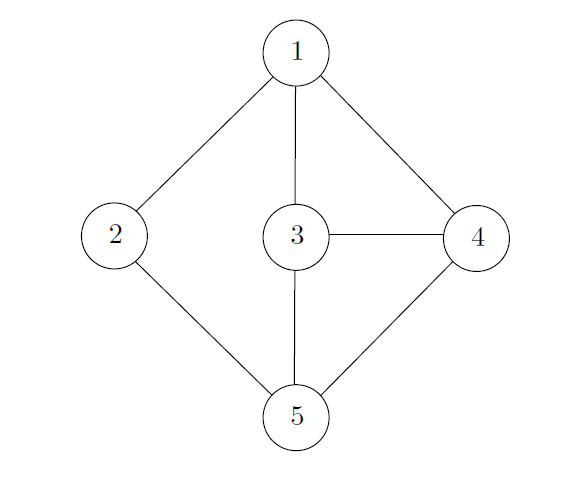
\includegraphics[width=\linewidth]{8-5.png}
	\caption{SIR Evolution Graph} 
	\label{Q8.5 Graph}
\end{figure}

Given a network (shown in Figure \ref{Q8.5 Graph}), the matrix $\mathbf{C}$ is given by
\[
	\mathbf{C} = \begin{bmatrix}
		0.375 & 0.0 & 0.0 & 0.0 & -0.125 \\
		0.0 & 0.75 & -0.25 & -0.25 & 0.0 \\
		0.0 & -0.25 & 0.417 & 0.083 & 0.0 \\
		0.0 & -0.25 & 0.083 & 0.417 & 0.0 \\
		-0.125 & 0.0 & 0.0 & 0.0 & 0.375
	\end{bmatrix}
\]

Given the formulation 
\[
	C_I(i) = \frac{1}{C_{ii} + (T + 2R) / N}
\]
it is easy to see that the Information Centrality measures information which "walks" through the entire network. The measure also penalizes nodes which information takes a long time to pass through as seen from the fact that the diagonals of $\mathbf{C}$ has higher values for those nodes that take comprise longer paths (Node 2 for example. Node 2 is connected but the paths which pass through it are usually not the geodesic paths).
\end{document}
